\documentclass[preprint]{aastex}
%\documentclass{emulateapj}
\usepackage[utf8]{inputenc}
\bibliographystyle{apj.bst} 
\newcommand{\meth}{CH$_4$}
\newcommand{\wat}{H$_2$O}
\newcommand{\Msun}{M$_\sun$}

\title{Progress Report: Brown Dwarfs Identified in WFC3 Infrared Spectroscopic Surveys}
\author{Christian Aganze \& Adam Burgasser}
\affil{Center for Astrophysics and Space Science, University of California San Diego }
\affil{9500 Gilman Dr, La Jolla, CA 92093}

\begin{document}

\maketitle

\section{Background}

Our understanding of the spatial distribution of brown dwarfs ( late M, L and T dwarfs with masses \textless 0.08 \Msun , \citealt{2005ARA&A..43..195K} ) beyond the local Solar Neighborhood is crucial for learning about their formation and their dynamical evolution and furthering our knowledge of the history of the Milky Way Galaxy.  Wide-field red optical and infrared surveys (e.g. 2MASS, SDSS, WISE) have allowed measurements of the local density of brown dwarfs, but covered a relatively shallow ( $\sim$50 pc) volume. Galactic disk and halo model parameters (e.g scale height, scale length (\citealt{2009ApJ...695.1591P}, \citealt{2005ApJ...631L.159R}, \citealt{Konishi2014}, \citealt{Vledder2016})) and radial distributions of these low mass and low luminosity objects are not well-constrained by observations. More importantly, brown dwarfs are also excellent tracers of galactic structure due to their long lifetimes hence characterizing these objects will significantly enhance our understating of the galactic history of the Milky Way. In addition, halo populations of brown dwarf are of great interest because these usually old and fast-moving objects  have a different formation and evolution track compared to brown dwarfs identified in the disk (\citealt{2013ApJS..205....6M}; \citealt{2014MNRAS.437.1009P}; \citealt{0004-637X-787-2-126}). However, not many halo brown dwarfs have been characterized due to their low luminosities and spectroscopic studies of brown dwarfs using ground-based telescopes are inhibited by the sky in the infrared region. Therefore space telescopes such as Hubble Space Telescope (HST) are useful for conducting these studies for distant brown dwarfs. 

We use data from two infrared WFC3 surveys: the WFC3 Infrared Spectroscopic Parallel Survey (WISPS, \citealt{2010ApJ...723..104A} ) and 3D-HST (\citealt{momcheva2015})). These two surveys both provided low-resolution G102 grism spectra (($\lambda$ = 0.8-1.17 $\micron$, R$\sim$210) and G141 grism spectra($\lambda$ = 1.11-1.67  $\micron$, R $\sim$130) as well as photometry for $\sim$250,0000 objects. The WISP survey is a 1000-orbit HST survey covering $\sim$390 fields ($\sim$1500 square arcminutes) and 3D-HST and 3D-HST is a 248-orbit HST survey spanning $\sim$600 square arcminutes. Both surveys are parallel surveys as pointings are determined by other other HST surveys (AEGIS, COSMOS, GOODS-S, UKIDSS-UDS for 3D-HST and  Cosmic Origins Spectrograph (COS) fields from a survey of white dwarfs for 3D-HST). Previous studies (\citealt{stanway16}, \citealt{Vledder2016}) have attempted to select early M-dwarfs in different high-redshift galaxies surveys based on their colors, but have not identified many late M and L, T dwarfs because they are too faint. \citet{2012ApJ...752L..14M} serendipitously discovered 3 late T-dwarfs (Par130\_BEAM\_84, Par58\_BEAM\_110A and Par32\_BEAM\_79A in Fig. 2) in the WISP survey identified by the grism spectra. To build a larger sample of similar objects, we have used near infrared spectral indices tracing \wat  and  \meth  molecular features found in L and T-dwarfs ( \citealt{1999ApJ...519..802K}, \citealt{2000ASPC..212...65B}) to identify brown dwarfs in the index-index space.

\section{Method: Near Infrared Spectral Indices in the J and H bands}

We define 5 wavelength regions in the near-infrared J and H bands (between 1.1 and 1.7 $\micron$) and 10 indices (Table 1) that are calculated using median flux  ratios (equation (1)) sampling \meth and \wat  molecular features observed in L and T-dwarfs (\citealt{1999ApJ...519..802K}, \citealt{2000ASPC..212...65B}) (Fig. 2). To select brown dwarfs, we select regions in the index-index space where brown dwarfs are more likely to be found based on the trend followed by spectral templates from the Spex Prism Library (SPL, \citealt{2014arXiv1406.4887B}). For instance, in Fig. 3 index-2 is defined as the ratio $ \widetilde{F}_{[1.38, 1.43]}/ \widetilde{F}_{[1.15, 1.20] }$ and index-5 is defined as the ratio  $ \widetilde{F}_{[1.38, 1.43] }/ \widetilde{F}_{ [1.246, 1.295]}$. To select brown dwarfs, we apply cuts in each index-index space creating selection criteria that are displayed in Table 2.

\begin{equation}
    index=\frac{\widetilde{F}_{[W1, W2]}}{\widetilde{F}_{[W3, W4]}}
\end{equation}

We also estimate completeness and contamination factors for each of the selection criteria per spectral type range. These values are given in equations (2) and (3) with $S_{WFC3}$ representing the number of selected sources in the field, $B_{WFC3}$ the number of selected sources that are M, L and T-dwarfs, and $WFC3_{tot}$ the total number of sources in the field. In equation (2) $S_{SPL}$ denotes the number of selected SPL templates, and $SPL_{tot}$ denotes the total number of spectra in SPL. Table 2 lists completeness and contamination factors for all 11 selection criteria for all spectral type ranges. We use low-contamination and high-completeness indices to select brown dwarfs within a spectral type range. For instance, we use c7 to find M5-L5 brown dwarfs with contamination \textless 37\% and completeness $\geq$ 99\%; and c1 to discover late T-dwarfs ($\geq$ T5) with contamination \textless 6\% and completeness $\geq$ 99\%. For selected sources, we use snr \textgreater 2 cutoff and chi-square  statistic (\citealt{2010ApJS..190..100K}) cutoff \textless 500,  estimated by fitting SPL templates from \citet{2014arXiv1406.4887B}. We finally conduct a visual inspection of the spectrum fitted to the best-fit standard to confirm the spectral type of each selected source.

\begin{equation}
    Contamination= \frac{(S_{WFC3}-B_{WFC3})}{WFC3_{tot}}\times 100
\end{equation}

\begin{equation}
    Completeness= \frac{S_{SPL}}{SPL_{tot}}\times 100
\end{equation}



\section{Preliminary Results}

We have found $\sim$48 M, L, T dwarfs by searching $\sim$350 fields in the WISP Survey and estimated their distances (Fig. 5) by calculating their absolute MKO magnitudes using absolute magnitudes and spectral types relations from \citet{2012ApJS..201...19D}  valid for all M6-T9 brown dwarfs. We then comparing these to their apparent MKO H magnitudes derived from their F110W, F160W and F140W magnitudes and their colors. In the future, we will expand this method to other WFC3 surveys such as HST-3D ( AEGIS, COSMOS, UDS and GOODS) to increase our sample. In addition, we will apply a machine learning clustering algorithms in a 10-dimensional index space to optimize our selection criteria and obtain a more robust measurement of our completeness and contamination statistics. We will also expand our training set to include subdwarf standards since these can present different spectral features in the J/H bands (\citealt{2007ApJ...669.1235L}). After these analyses, we will use  Markov Chain Monte Carlo (MCMC) code with a Metropolis-Hastings algorithm (\citealt{1953JChPh..21.1087M}; \citealt{HASTINGS01041970}) to fit galactic disk and halo density models to the number the number of brown dwarfs and distances to further constrain model parameters such as scale height and scale length.
\clearpage
\begin{figure}[!htb]
\center
\epsscale{2}
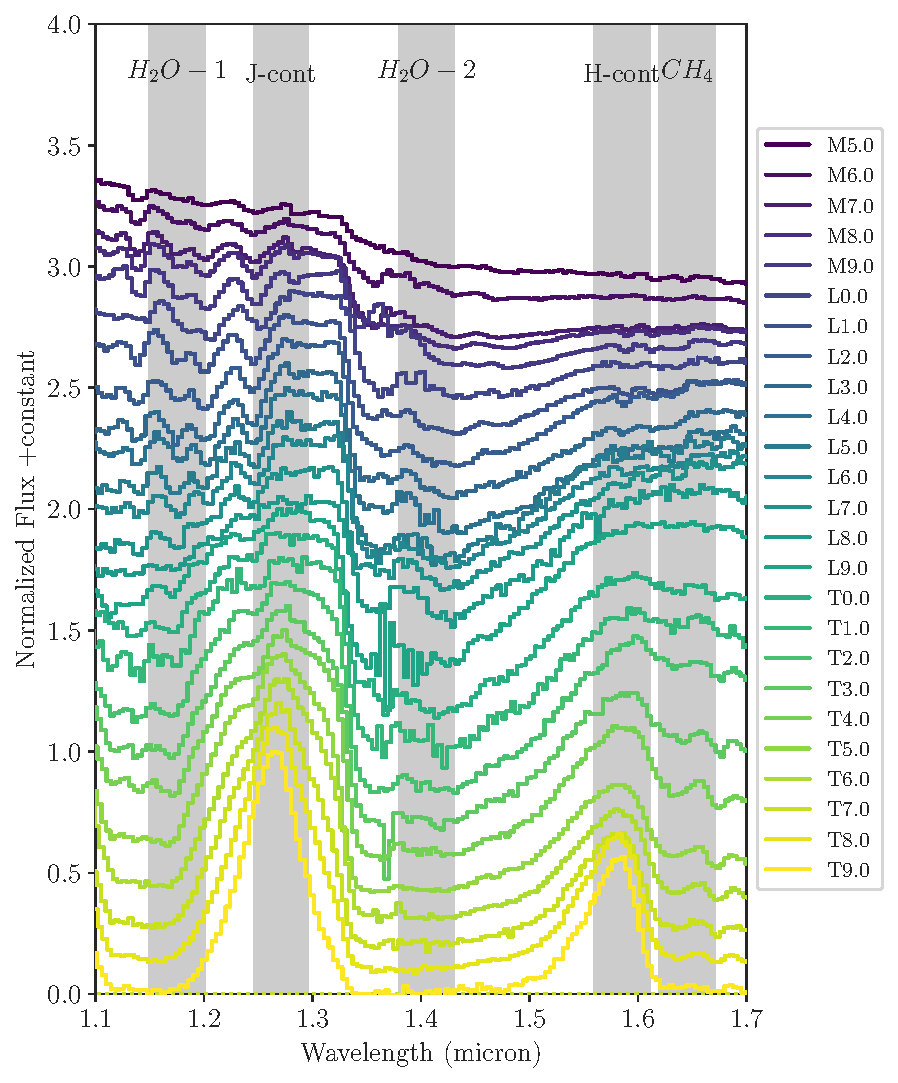
\includegraphics[width=0.8\textwidth]{../Figures/standards.pdf}
\figurenum{1}
\caption{ L0-T9 spectral standards (\citealt{2010ApJS..190..100K}) with nir bands that we use to define indices highlighted }
\end{figure}
\clearpage
\begin{figure}[!htb]
\center
\epsscale{3}
\includegraphics[width=1\textwidth]{../Figures/indexplot.pdf}
\figurenum{2}
\caption{Index-2 vs Index-9 plotting SPL known brown dwarfs, brown dwarfs in the previously found in WISP survey and a few ''contaminants". Sources that lie below the black line will be selected by c6 (Table 2 )
 }
 \end{figure}
\clearpage
\begin{figure}[!htb]
\center
\epsscale{1}
\includegraphics[width=0.75\textwidth]{../Figures/wispbds.pdf}
\figurenum{3}
\caption{ Spectra of discovered of L and T dwarfs, names are formatted by WISPS field name and object number; and nir bands used to define indices and main absorption features are highlighted}
\end{figure}

\clearpage
\begin{figure}[!htb]
\center
\epsscale{2}
\includegraphics[width=0.9\textwidth]{../Figures/distances.pdf}
\figurenum{4}
\caption{ Photometric distances for found brown dwarfs computed using absolute magnitude/spectral types relations from \citet{2012ApJS..201...19D}. All spectral types are estimated by fitting to spectral standards. 15=M5.0}
\end{figure}

\clearpage
\begin{table}
\center
\begin{tabular}{llrrrrrr}
\\ \hline \hline \\
    Index & Definition \\
\\ \hline \hline \\
    index1 & $ \widetilde{F}_{[1.246, 1.295]}/ \widetilde{F}_{[1.15, 1.20]}$ \\
    index2 & $ \widetilde{F}_{[1.38, 1.43]}/ \widetilde{F}_{[1.15, 1.20] }$\\
    index3 & $ \widetilde{F}_{[1.56, 1.61]}/ \widetilde{F}_{[1.15, 1.20]}$ \\
    index4 & $ \widetilde{F}_{[1.62,1.67]}/ \widetilde{F}_{[1.15, 1.20]}$ \\
    index5 & $ \widetilde{F}_{[1.38, 1.43] }/ \widetilde{F}_{ [1.246, 1.295]}$ \\
    index6 & $ \widetilde{F}_{[1.56, 1.61] }/ \widetilde{F}_{[1.246, 1.295]}$\\
    index7&  $ \widetilde{F}_{[1.62,1.67]}/ \widetilde{F}_{[1.246, 1.295]}$\\
    index8 & $ \widetilde{F}_{[1.56, 1.61]}/ \widetilde{F}_{[1.38, 1.43]}$\\
    index9 & $ \widetilde{F}_{[1.62,1.67]}/ \widetilde{F}_{[1.38, 1.43]}$ \\
    index10 & $ \widetilde{F}_{ [1.62,1.67]}/ \widetilde{F}_{[1.56, 1.61]}$\\
    
\\ \hline \hline \\
\end{tabular}
\caption{List of indices computed using median flux ratios, these wavelength ranges are also highlighted in Fig. 1}
\end{table}


\clearpage
\begin{table}
\center
\begin{tabular}{llrrrrrr}
\\ \hline \hline \\
    Criterion & index-index Space & Selection Condition \\
\\ \hline \hline \\
    c1 &Any &  i1 \textgreater2.5 \\
    c2 & Any &  i3  \textgreater1.9  \\
    c3 & Any &  i8  \textgreater7.0  \\
    c4 &Any &  i9   \textgreater2.0   \\
    c5 & Any &  i5  \textless 0.6   \\
    c6 & index2 vs index5 & (index5-0.2 ) $\geq$ (0.8/0.9)$\times$ (index4-0.1)\\
    c7 & index4 vs index6 & (index6-0.15)  $\geq$ (0.48/0.85) $\times$ (index4-0.5) \\
    c8 & index4 vs index7 & (index7-0.1)  $\geq$ 1.1\ $\times$ (index4-0.25)\\
    c9 & index5 vs index6 & (index6-0.1) $\leq$ (0.9/0.7)$\times$ (index5-0.3)  \\
    c10 &index2 vs index4 &  index4 $\leq$ (1/0.6) $\times$ index4 or index4 \textless 1.0 \\
    c11 & index4 vs index5 &  index5 \textless 0.5 or  index4 \textgreater 1.2 \\
\\ \hline \hline \\
\end{tabular}
\caption{ Definition of selection criteria defined using indcies defined in Table 1}
\end{table}


\clearpage
\begin{table}
\center
\begin{tabular}{llrrrrrr}
\\ \hline \hline \\
  Selection Criterion &  Contamination & \multicolumn{5}{c|}{Completeness} \\
  \hline \\
  & &  M5.0-M9.9 & L0.0-L4.9 &  L5.0-L9.9 &  T0.0-T5 &  T5-Y0\\
\\ \hline \hline \\
   c1 &              6 &          0 &          0 &          0 &       15 &     \textbf{99} \\
   c2 &              9 &          0 &          1 &          0 &        2 &     69 \\
   c3 &              2 &          0 &          0 &          0 &       10 &     65\\ 
   c4&             10 &          4 &         55 &          0 &       \textbf{95} &     76 \\ 
   c5 &             65 &          1 &          0 &          7 &       47 &    100 \\
   c6 &             86 &        100 &        100 &        100 &      100 &     93 \\   
   c7 &             37 &         \textbf{99} &        \textbf{100} &         99 &      100 &     99 \\ 
   c8 &             45 &        100 &        100 &        100 &      100 &    100 \\  
   c9 &             47 &          0 &          0 &          0 &       67 &     99 \\ 
   c10 &             57 &         40 &         94 &          2 &       72 &     19 \\
   c11 &             64 &         3 &         33 &          95 &       100 &     100\\
\\ \hline \hline \\
\end{tabular}
\caption{Table showing completeness and contamination computed using equations (2) and (3) for each spectral type range for selection criteria described in Table 2. The best indices (low-contamination, high completeness) are in bold}
\end{table}

\clearpage
\bibliography{library.bib}
\end{document}


